% General statement: why gradients are important?
Evaluating how changes in the parameter of a certain function plays a central role in optimization, sensitivity analysis, Bayesian inference, uncertainty quantification, among others. 
Modern machine learning applications require the use of gradients to exploit more efficiently the space of parameters. 
When optimizing a loss function, gradient-based methods (for example, gradient descent and its many variants \cite{ruder2016overview-gradient-descent}) are more efficient at finding minimal and converge faster to them than than gradient-free methods.
When numerically computing the posterior of a probabilistic model, gradient-based sampling strategies converge faster to the posterior distribution than gradient-free methods. 
Second derivatives further help to improve convergence rates of these algorithms and allow uncertainty quantification around parameter values. 

% Differential equations
Dynamical systems where the goal is to model observations governed by differential equations is not an exception to the rule.
In the field of statistics, the sensitivity equations provide a way to compute gradients of a given loss function with respect to the parameters of the dynamical system, which can be used for estimation of the parameters. 
In numerical analysis, the estimation of the gradient can be used to understand how sensitive is the solution of a differential equation to a parameter. 
In recent years, there has been an increasing interest in designing machine learning pipelines that include constraints to the physical system in the form of differential equations. Examples of this include physics-informed neural networks (PINNs) \cite{PINNs_2019} and universal differential equations (UDEs) \cite{rackauckas2020universal}.  
% soft / hard constrains

% Differentiation 
However, when working with differential equations the computation of gradients is not an easy task, both regarding the mathematical framework and software implementation involved. 
Except for a small set of particular cases, most differential equations require numerical methods to estimate their solution. 
This means that solutions cannot be directly differentiated and require special treatment if, besides the numerical solution, we want to extract first or second order derivatives. 
Furthermore, numerical solutions introduce approximation errors and these errors can be propagated and even amplified during the computation of the gradient. 
On the other side, there is a broad literature in numerical methods for solving differential equations. 
If well each method provides different guarantees and advantages depending the use case, this means that the tools developed to compute gradients when using a solver need to be universal enough in order to apply to all or at least a large set of these. 
The first goal of this article is making a review of the different methods that exists to archive this goal.
\begin{quote}
    \textbf{Question 1. }
    \textit{How can we compute the gradient of a function that depends on the numerical solution of a differential equation?}
\end{quote}
Notice here the phrasing \textit{the gradient of a function that depends}, emphasizing the fact that in many cases we may be interested in computing the gradient of a function that depends on the solution of the differential equation.
This is certainly the case in machine learning and optimization where the goal is to minimize a loss function that depends of some predicted and target responses. 

% AD
The broader set of tools known as Automatic Differentiation (AD) aims to compute derivatives by sequentially applying the chain rule the the sequence of unit operations that compose a computer program. 
The premise is simple: every program, including a numerical solver, is ultimately described by a long chain of simple algebraic operations (addition, multiplication) that are i) easy to differentiate and ii) their combination is easy to differentiate by using the chain rule. 
If well many modern applications use AD at some extend, there is also a family of methods that compute the gradient by relying in a secondary set of differential equations. 
We are going to refer to this family of methods as \textit{continuous}, and we will dedicate them a special treatment in future sections to distinguish them from the discrete algorithms that resemble more to pure AD. 

The difference between the different methods encapsulates both their formulation and implementation in different software, but also their serve different objectives too. 
Different methods have different computational complexities depending the number of parameters and differential equations, and these complexities are also balanced between total execution time and required memory. 
The second goal of this work is then to illustrate the different advantages and limitations of this methods, and how to use them in modern scientific software. 
\begin{quote}
    \textbf{Question 2. }
    \textit{What are the pros and cons of these methods and how can I implement them in my research?}
\end{quote}
If well these methods can be (in principle) implemented in different programming languages, here we decided to use the Julia programming language for the different examples. 
Julia is a recently new and mature programming language that has already a large tradition in implementing packages aiming to advance differential programming \cite{Julialang_2017}. 

% The need to introduce all this methods in a common framework
Without aiming at making an extensive and specialized review on the field, we find this resource useful for other researchers and students working on problems that combine optimization and sensitivity analysis with differential equations.
Differential programming is opening new ways  
\begin{quote}
    \textbf{Question 3. }
    \textit{What are the new opportunities in embracing these tools?}
\end{quote}

\subsection{Use cases}

\subsection{Some basic jargon}

\section{General formulation}


Consider a system of ordinary differential equations given by
\begin{equation}
 \frac{du}{dt} = f(u, \theta, t),
 \label{eq:original_ODE}
\end{equation}
where $u \in \mathbb{R}^n$, $\theta \in \mathbb R^p$, and initial condition $u(t_0) = u_0$.
Here $n$ denotes the total number of ordinary differential equations and $p$ the size of a parameter embedded in the functional form of the differential equation.
Although we consider here the case of ordinary differential equations, that is, when the derivatives are just with respect to the time variable $t$, we will later include the case of partial differential equations (PDE).
We are interested in computing the gradient of a given loss function $L(u(\cdot, \theta))$ with respect to the parameter $\theta$.
Examples of loss functions include
\begin{equation}
 L(u(\cdot, \theta)) = \| u(t_1, \theta) - u_1 \|_2^2,
\end{equation}
where $u_1$ is the desired target observation at some later time $t_1$; and
\begin{equation}
 L(u(\cdot, \theta)) = \int_{t_0}^{t_1} h( u(t;\theta), \theta) ) dt, 
\end{equation}
with $h$ some function that quantifies the contribution of the error term at time $t \in [t_0, t_1]$.
We are interested in computing the gradient of the loss function with respect to the parameter $\theta$, which can be written as
\begin{equation}
 \frac{dL}{d\theta} = \frac{dL}{du} \frac{du}{d\theta}.
 \label{eq:dLdtheta_VJP}
\end{equation} 
The first term is usually easy to evaluate, since it just involves the partial derivative of the scalar loss function to the solution.
The second term on the right hand side is the actual bottleneck and it is usually referred to as the sensitivity,
\begin{equation}
 s = \frac{\partial u}{\partial \theta} \in \mathbb R^{n \times p}.
\end{equation}

\begin{figure}[]
    \centering
    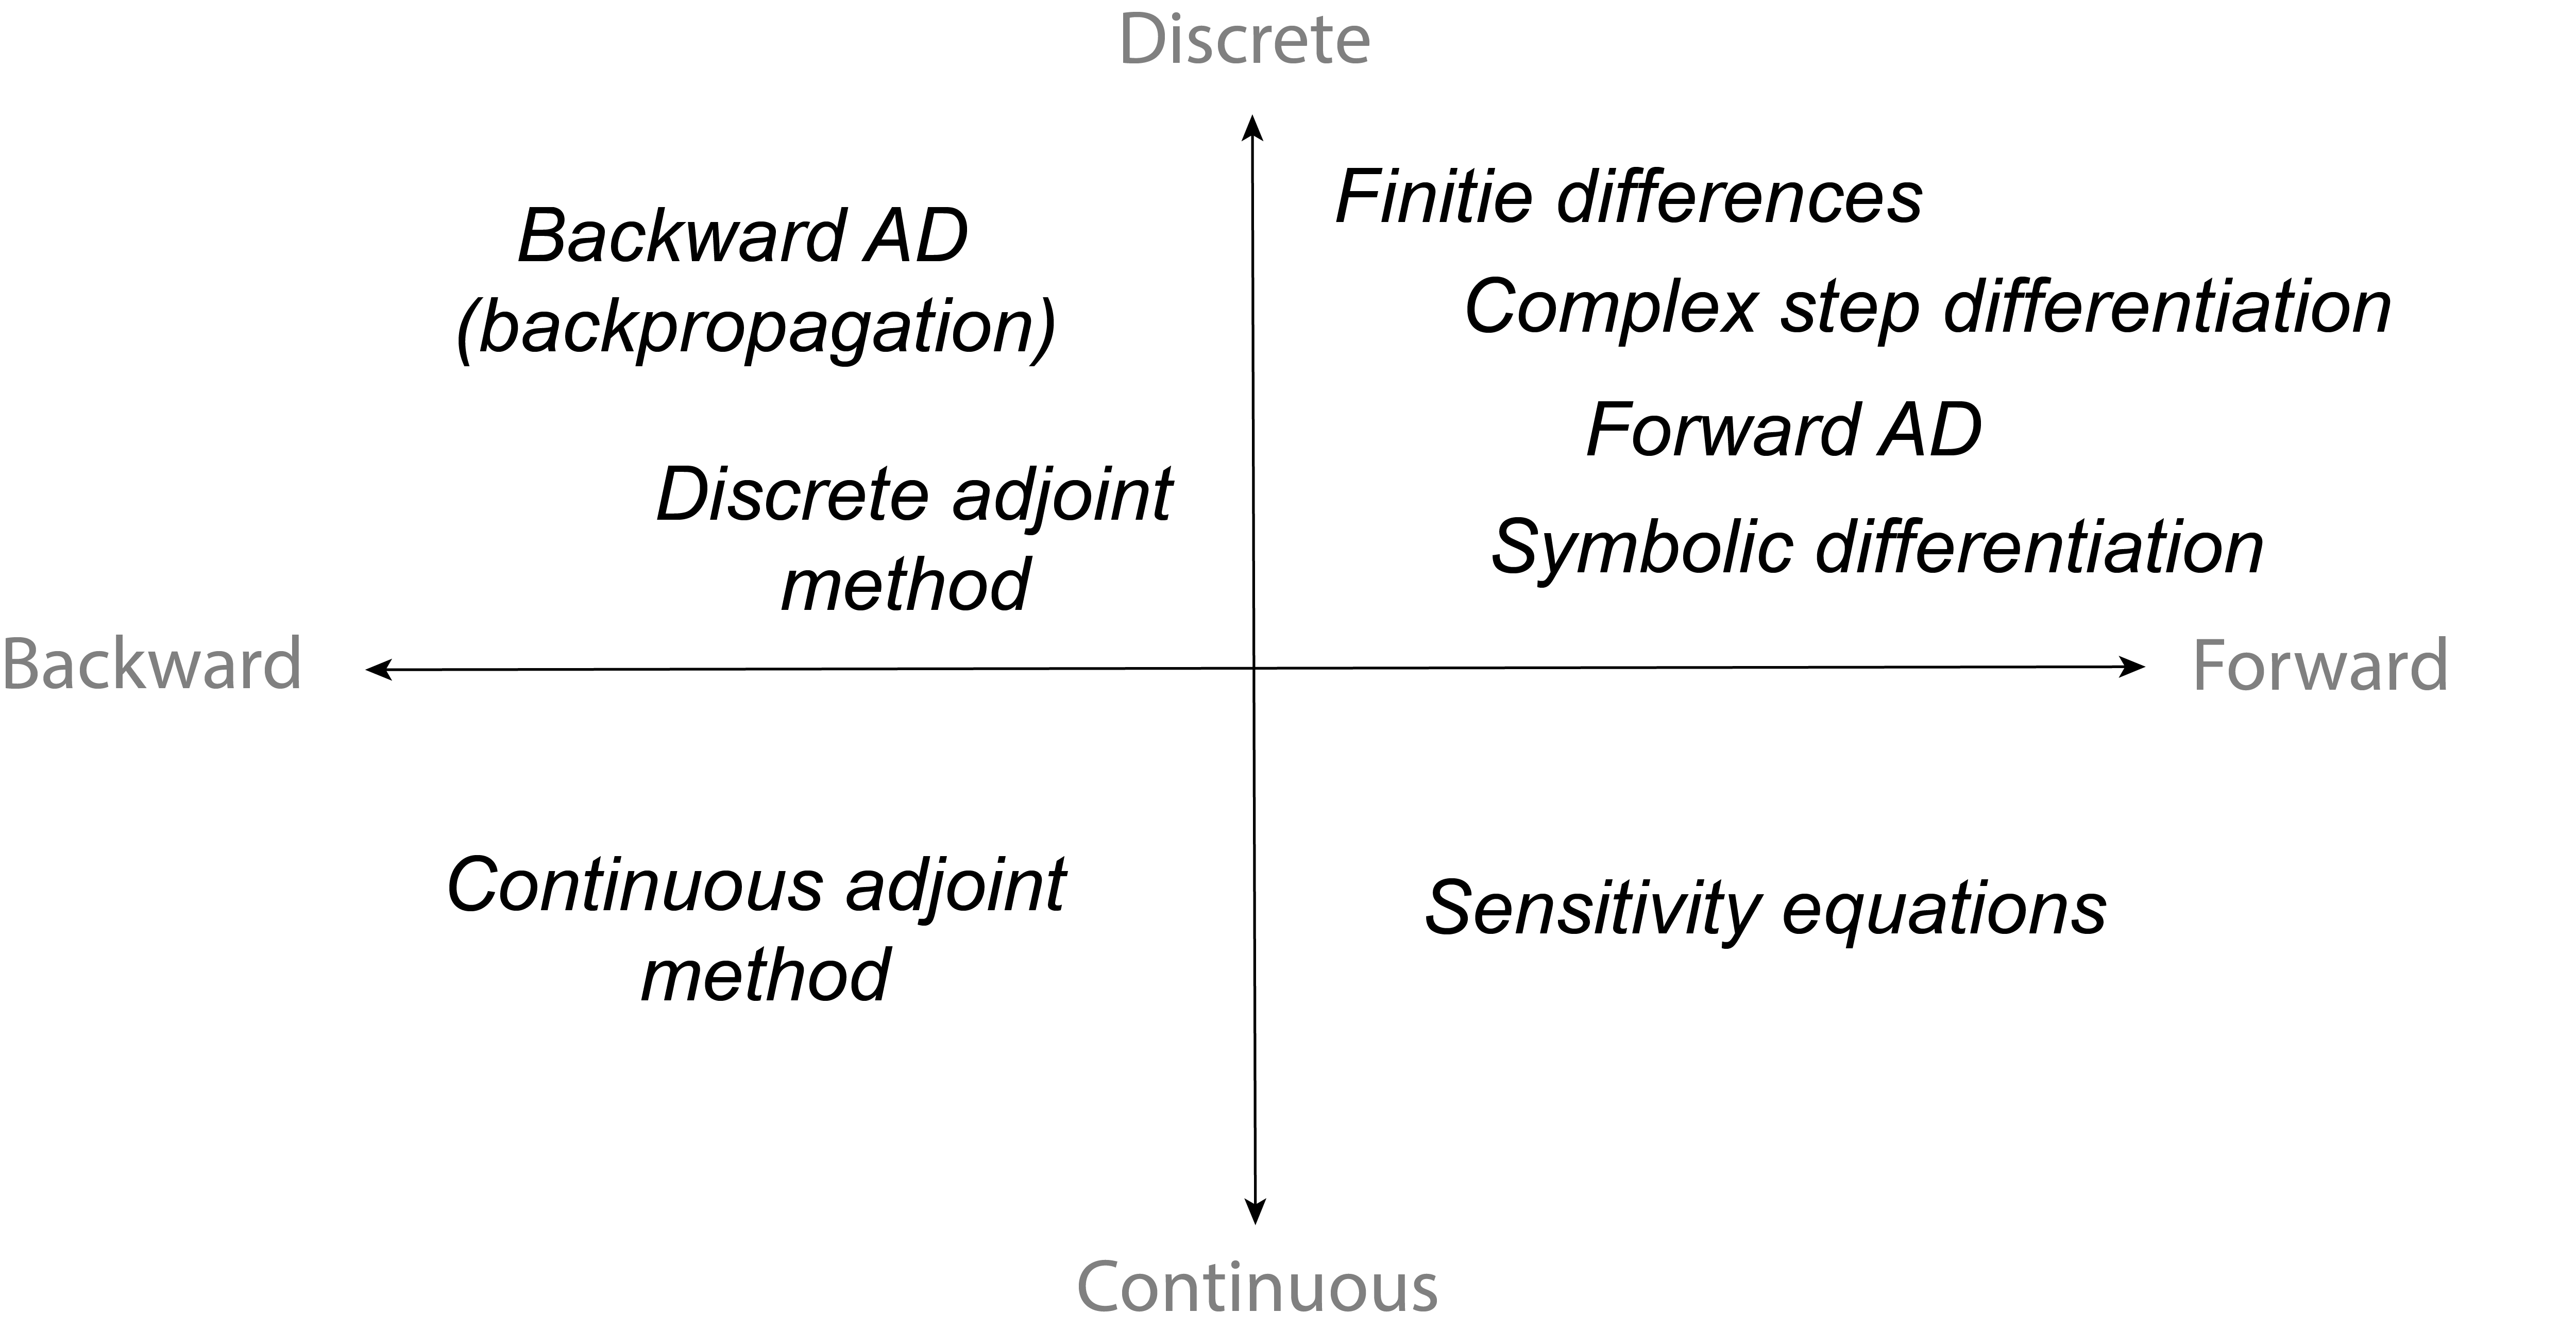
\includegraphics[width=0.80\textwidth]{figures/scheme-methods.png}
    \caption{Schematic representation of the different methods available for differentiation involving differential equation solutions.}
    \label{fig:diff}
\end{figure}
Depending on the number of parameters and the complexity of the differential equation we are trying to solve, there are different methods to compute gradients with different numerical and computational advantages and that also scale differently depending of the number of differential equations $n$ and number of parameters $p$.
These methods can be roughly classified as:
\begin{itemize}
    \item \textit{Discrete} vs \textit{continuous} methods.
    \item \textit{Forward} vs \textit{backwards} methods.
\end{itemize}
The first difference regards the fact that the method for computing the gradient can be either based on the manipulation of atomic operations that are easy to differentiate using the chain rule several times (discrete), in opposition to the approach of approximating the gradient as the numerical solution of a new set of differential equations (continuous).
The second distinction is related to the fact that some methods compute gradients by resolving a new sequential problem that may move in the same direction of the original numerical solver - i.e. moving forward in time - or, instead, they solve a new system that goes backwards in time. 
Figure \ref{fig:diff} displays a classification of some methods under this two-fold classification. In the following section we are going to explore more in detail these methods.